
\begin{center}
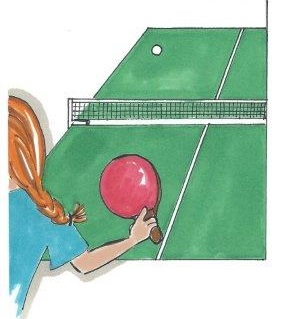
\includegraphics[width=0.5\textwidth]{content/3/chapter7/images/1.png}\\
Cippi在打乒乓球
\end{center}

\begin{tcolorbox}[breakable,enhanced jigsaw,colback=blue!5!white,colframe=blue!75!black,title={The Reference PCs}]
You should take the performance numbers with a grain of salt. I’m not interested in the exact number for each variation of the algorithms on Linux and Windows. I’m more interested in getting a gut feeling of which algorithms may work and which algorithms may not work. I’m not comparing the absolute numbers of my Linux desktop with the numbers on my Windows laptop, but I’m interested to know if some algorithms work better on Linux or Windows.
\end{tcolorbox}

When you want to synchronize threads more than once, you can use condition variables, std::atomic\_flag, std::atomic<bool>, or semaphores. In this section, I want to answer the question: which variant is the fastest?

To get comparable numbers, I implement a ping-pong game. One thread executes a ping function (or ping thread for short), and the other thread a pong function (or pong thread for short). The ping thread waits for the pong-thread notification and sends the notification back to the pong thread. The game stops after 1,000,000 ball changes. I perform each game five times to get comparable performance numbers.

\begin{tcolorbox}[breakable,enhanced jigsaw,colback=blue!5!white,colframe=blue!75!black,title={About the Numbers}]
I made my performance test at the end of 2020 with the brand new Visual Studio compiler 19.28 because it already supported synchronization with atomics (std::atomic\_flag and std::atomic) and semaphores. Additionally, I compiled the examples with maximum optimization (/Ox). The performance number should only give a rough idea of the relative performance of the various ways to synchronize threads. When you want the exact number on your platform, you have to repeat the tests.
\end{tcolorbox}

Let me start the comparison with C++11.

\subsubsubsection{7.1.1\hspace{0.2cm} Condition Variables}

\hspace*{\fill} \\ %插入空行
\noindent
Multiple time synchronization with a condition variable
\begin{lstlisting}[style=styleCXX]
// pingPongConditionVariable.cpp

#include <condition_variable>
#include <iostream>
#include <atomic>
#include <thread>

bool dataReady{false};

std::mutex mutex_;
std::condition_variable condVar1;
std::condition_variable condVar2;

std::atomic<int> counter{};
constexpr int countlimit = 1'000'000;

void ping() {

	while(counter <= countlimit) {
		{
			std::unique_lock<std::mutex> lck(mutex_);
			condVar1.wait(lck, []{return dataReady == false;});
			dataReady = true;
		}
		++counter;
		condVar2.notify_one();
	}
}

void pong() {

	while(counter < countlimit) {
		{
			std::unique_lock<std::mutex> lck(mutex_);
			condVar2.wait(lck, []{return dataReady == true;});
			dataReady = false;
		}
		condVar1.notify_one();
	}

}

int main(){

	auto start = std::chrono::system_clock::now();
	
	std::thread t1(ping);
	std::thread t2(pong);
	
	t1.join();
	t2.join();
	
	std::chrono::duration<double> dur = std::chrono::system_clock::now() - start;
	std::cout << "Duration: " << dur.count() << " seconds" << '\n';
}
\end{lstlisting}

I use two condition variables in the program: condVar1 and condVar2. The ping thread waits for the notification of condVar1 and sends its notification with condVar2. Variable dataReady protects against spurious and lost wakeups. The ping-pong game ends when counter reaches the countlimit. The notify\_one calls (lines 26 and 38) and the counter are thread-safe and are, therefore, outside the critical region.

Here are the numbers.

\begin{center}
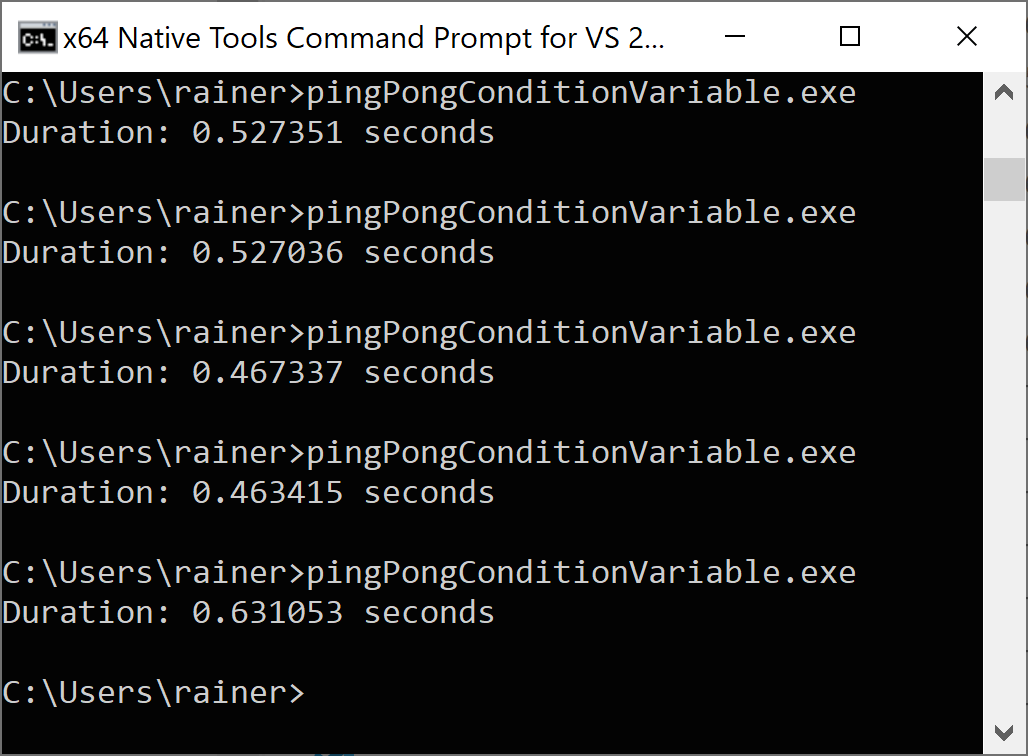
\includegraphics[width=0.8\textwidth]{content/3/chapter7/images/2.png}\\
Multiple time synchronizations with condition variables
\end{center}

The average execution time is 0.52 seconds.

Porting this workflow to std::atomic\_flag in C++20 is straightforward.

\subsubsubsection{7.1.2\hspace{0.2cm} std::atomic\_flag}

Here is the same workflow using two atomic flags and then one.

\hspace*{\fill} \\ %插入空行
\noindent
\textbf{7.1.2.1\hspace{0.2cm} Two Atomic Flags}

In the following program, I replace the waiting on the condition variable with the waiting on the atomic flag and the condition variable’s notification with the atomic-flag setting followed by the notification.

\hspace*{\fill} \\ %插入空行
\noindent
Multiple time synchronization with two atomic flags
\begin{lstlisting}[style=styleCXX]
// pingPongAtomicFlags.cpp

#include <iostream>
#include <atomic>
#include <thread>

std::atomic_flag condAtomicFlag1{};
std::atomic_flag condAtomicFlag2{};

std::atomic<int> counter{};
constexpr int countlimit = 1'000'000;
void ping() {
	while(counter <= countlimit) {
		condAtomicFlag1.wait(false);
		condAtomicFlag1.clear();
		
		++counter;
		
		condAtomicFlag2.test_and_set();
		condAtomicFlag2.notify_one();
	}
}

void pong() {
	while(counter < countlimit) {
		condAtomicFlag2.wait(false);
		condAtomicFlag2.clear();
		
		condAtomicFlag1.test_and_set();
		condAtomicFlag1.notify_one();
	}
}

int main() {

	auto start = std::chrono::system_clock::now();
	
	condAtomicFlag1.test_and_set();
	std::thread t1(ping);
	std::thread t2(pong);
	
	t1.join();
	t2.join();
	
	std::chrono::duration<double> dur = std::chrono::system_clock::now() - start;
	std::cout << "Duration: " << dur.count() << " seconds" << '\n';

}
\end{lstlisting}

A call condAtomicFlag1.wait(false) (line 15) blocks if the atomic flag’s value is false, and returns if condAtomicFlag1 has the value true. The boolean value serves as a kind of predicate and must, therefore, be set back to false (line 15). Before the notification (line 21) is sent to the pong thread, condAtomicFlag1 is set to true (line 20). The initial setting of condAtomicFlag1 (line 39) to true starts the game.

Thanks to std::atomic\_flag, the game ends faster.

\begin{center}
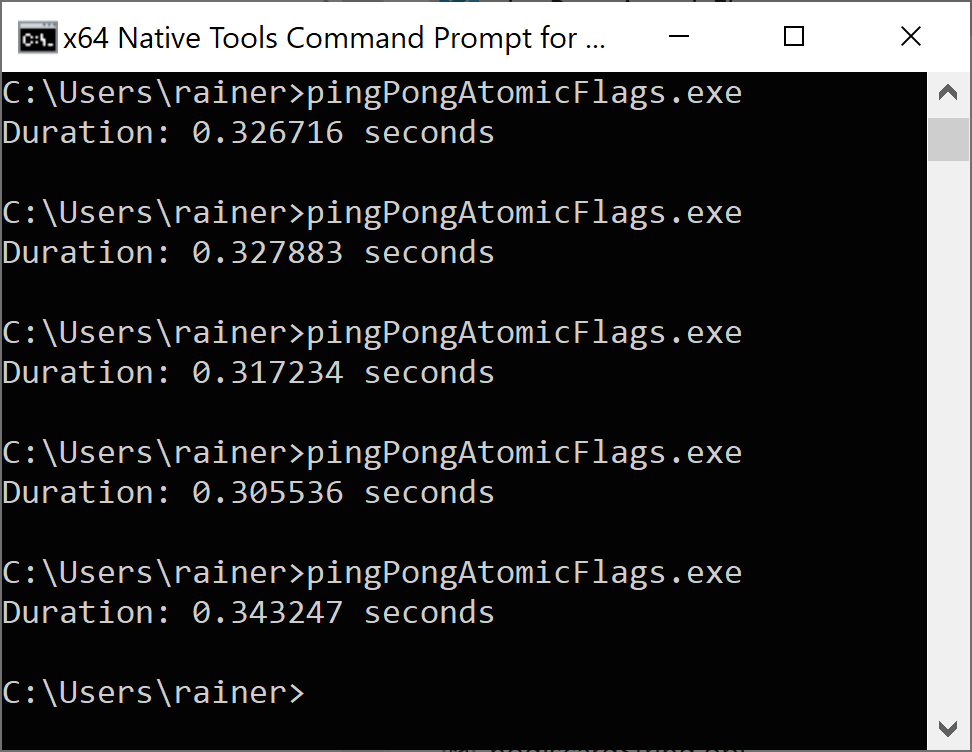
\includegraphics[width=0.8\textwidth]{content/3/chapter7/images/3.png}\\
Multiple time synchronization with two atomic flags
\end{center}

On average, a game takes 0.32 seconds.

When you analyze the program, you may recognize that one atomic flag is sufficient for the workflow.

\hspace*{\fill} \\ %插入空行
\noindent
\textbf{7.1.2.2\hspace{0.2cm} One Atomic Flag}

Using one atomic flag makes the workflow easier to understand.

\hspace*{\fill} \\ %插入空行
\noindent
Multiple time synchronization with one atomic flag
\begin{lstlisting}[style=styleCXX]
// pingPongAtomicFlag.cpp

#include <iostream>
#include <atomic>
#include <thread>

std::atomic_flag condAtomicFlag{};

std::atomic<int> counter{};
constexpr int countlimit = 1'000'000;

void ping() {
	while(counter <= countlimit) {
		condAtomicFlag.wait(true);
		condAtomicFlag.test_and_set();
		
		++counter;
		
		condAtomicFlag.notify_one();
	}
}

void pong() {
	while(counter < countlimit) {
		condAtomicFlag.wait(false);
		condAtomicFlag.clear();
		condAtomicFlag.notify_one();
	}
}

int main() {

	auto start = std::chrono::system_clock::now();
	
	condAtomicFlag.test_and_set();
	std::thread t1(ping);
	std::thread t2(pong);
	
	t1.join();
	t2.join();
	
	std::chrono::duration<double> dur = std::chrono::system_clock::now() - start;
	std::cout << "Duration: " << dur.count() << " seconds" << '\n';

}
\end{lstlisting}

In this case, the ping thread blocks on true but the pong thread blocks on false. From the performance perspective, using one or two atomic flags makes no difference.

\begin{center}
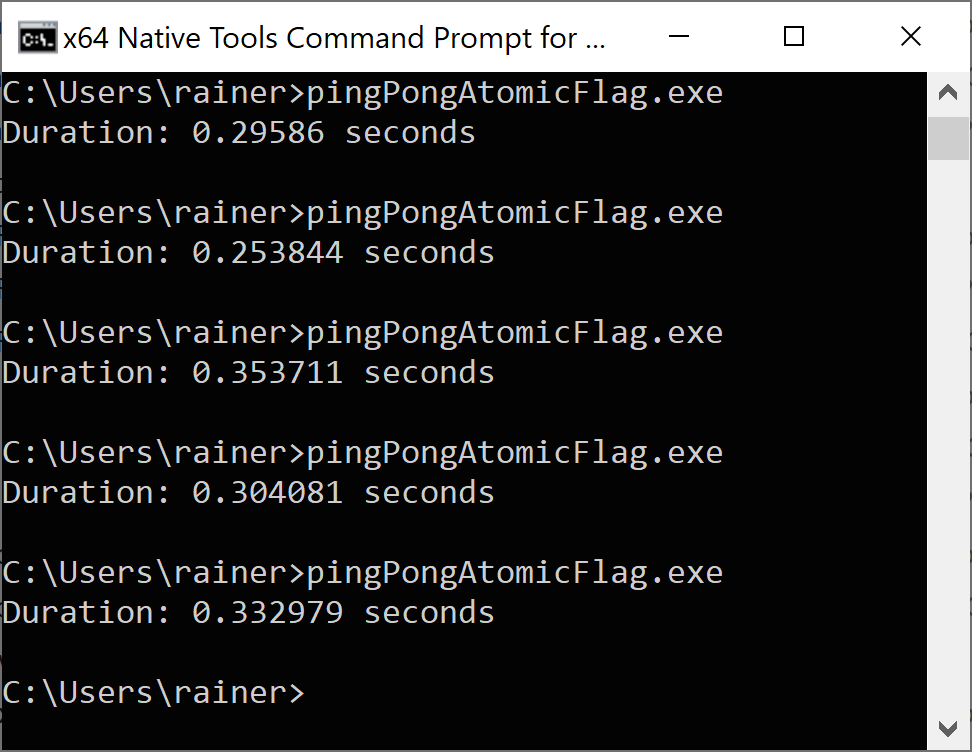
\includegraphics[width=0.8\textwidth]{content/3/chapter7/images/4.png}\\
Multiple time synchronization with one atomic flag
\end{center}

The average execution time is 0.31 seconds.

I used in this example std::atomic\_flag such as an atomic boolean. Let’s give it another try with std::atomic<bool>.

\subsubsubsection{7.1.3\hspace{0.2cm} std::atomic<bool>}

The following C++20 implementation is based on std::atomic.

\hspace*{\fill} \\ %插入空行
\noindent
Multiple time synchronization with an atomic bool
\begin{lstlisting}[style=styleCXX]
// pingPongAtomicBool.cpp

#include <iostream>
#include <atomic>
#include <thread>

std::atomic<bool> atomicBool{};

std::atomic<int> counter{};
constexpr int countlimit = 1'000'000;

void ping() {
	while(counter <= countlimit) {
		atomicBool.wait(true);
		atomicBool.store(true);
		
		++counter;
		
		atomicBool.notify_one();
	}
}

void pong() {
	while(counter < countlimit) {
		atomicBool.wait(false);
		atomicBool.store(false);
		atomicBool.notify_one();
	}
}

int main() {

	std::cout << std::boolalpha << '\n';
	
	std::cout << "atomicBool.is_lock_free(): "
	<< atomicBool.is_lock_free() << '\n';
	
	std::cout << '\n';
	
	auto start = std::chrono::system_clock::now();
	
	atomicBool.store(true);
	std::thread t1(ping);
	std::thread t2(pong);
	
	t1.join();
	t2.join();
	
	std::chrono::duration<double> dur = std::chrono::system_clock::now() - start;
	std::cout << "Duration: " << dur.count() << " seconds" << '\n';

}
\end{lstlisting}

std::atomic<bool> can internally use a locking mechanism such as a mutex. My Windows run time is lock-free.

\begin{center}
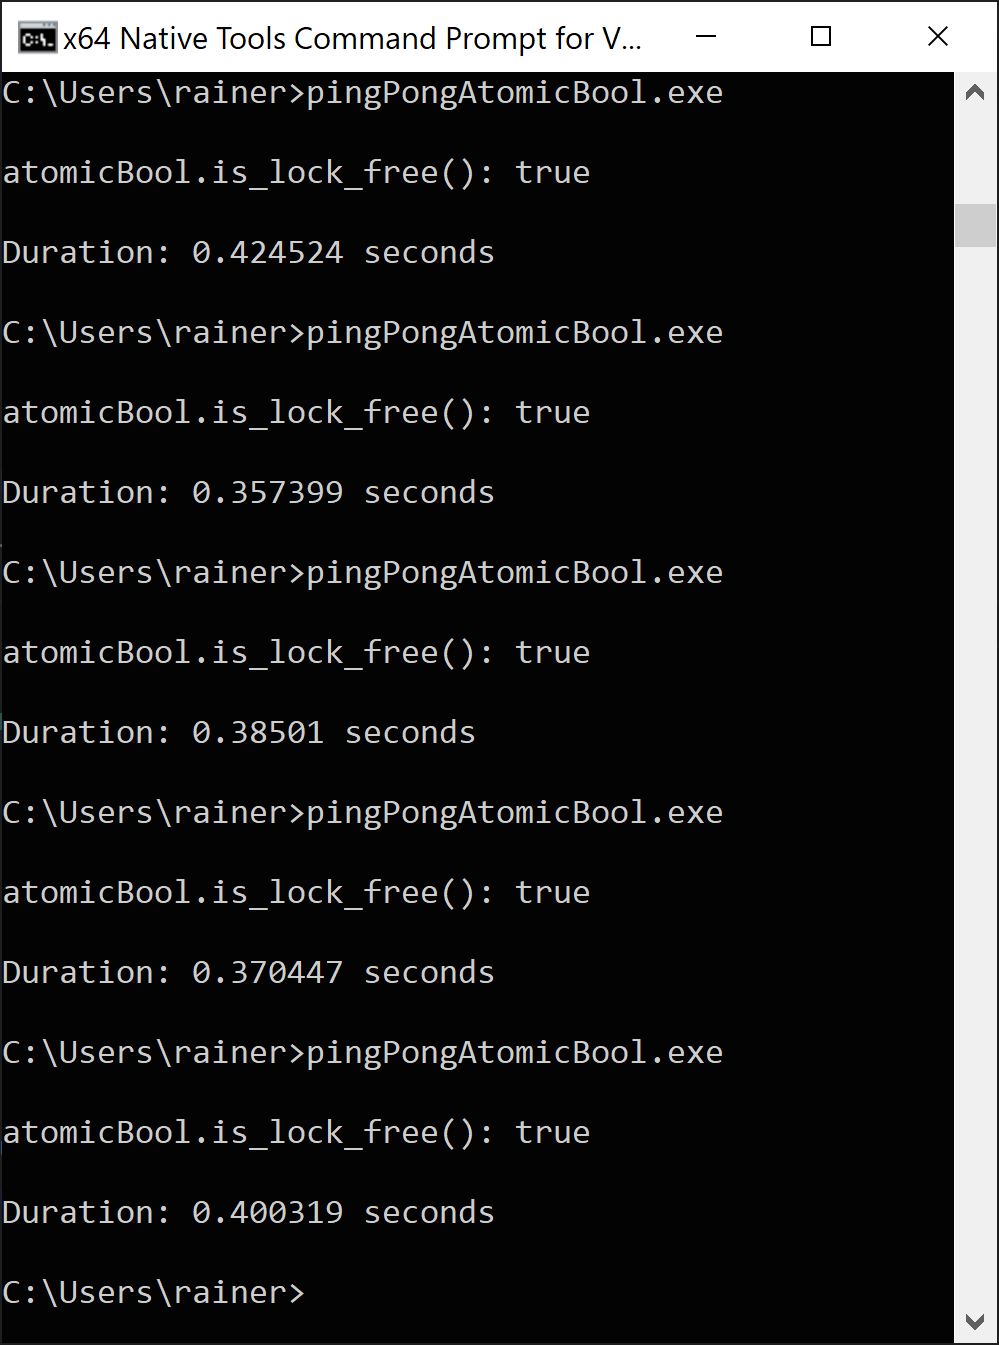
\includegraphics[width=0.8\textwidth]{content/3/chapter7/images/5.png}\\
Multiple time synchronization with an atomic bool
\end{center}

On average, the execution time is 0.38 seconds.

From the readability perspective, this implementation based on std::atomic is straightforward to understand. This observation also holds for the next implementation of the ping-pong game based on semaphores.

\subsubsubsection{7.1.4\hspace{0.2cm} Semaphores}

Semaphores promise to be faster than condition variables. Let’s see if this is true.

\hspace*{\fill} \\ %插入空行
\noindent
Multiple time synchronization with semaphores
\begin{lstlisting}[style=styleCXX]
// pingPongSemaphore.cpp

#include <iostream>
#include <semaphore>
#include <thread>

std::counting_semaphore<1> signal2Ping(0);
std::counting_semaphore<1> signal2Pong(0);

std::atomic<int> counter{};
constexpr int countlimit = 1'000'000;

void ping() {
	while(counter <= countlimit) {
		signal2Ping.acquire();
		++counter;
		signal2Pong.release();
	}
}

void pong() {
	while(counter < countlimit) {
		signal2Pong.acquire();
		signal2Ping.release();
	}
}

int main() {

	auto start = std::chrono::system_clock::now();
	
	signal2Ping.release();
	std::thread t1(ping);
	std::thread t2(pong);
	
	t1.join();
	t2.join();
	
	std::chrono::duration<double> dur = std::chrono::system_clock::now() - start;
	std::cout << "Duration: " << dur.count() << " seconds" << '\n';

}
\end{lstlisting}

The program pingPongsemaphore.cpp uses two semaphores: signal2Ping and signal2Pong (lines 7 and 8). Both can have the two values 0 or 1, and are initialized with 0. This means when the value is 0 for the semaphore signal2Ping, a call signal2Ping.release() (lines 24 and 32) sets the value to 1 and is, therefore, a notification. A signal2Ping.acquire() (line 15) call blocks until the value becomes 1. The same argumentation holds for the second semaphore signal2Pong.

\begin{center}
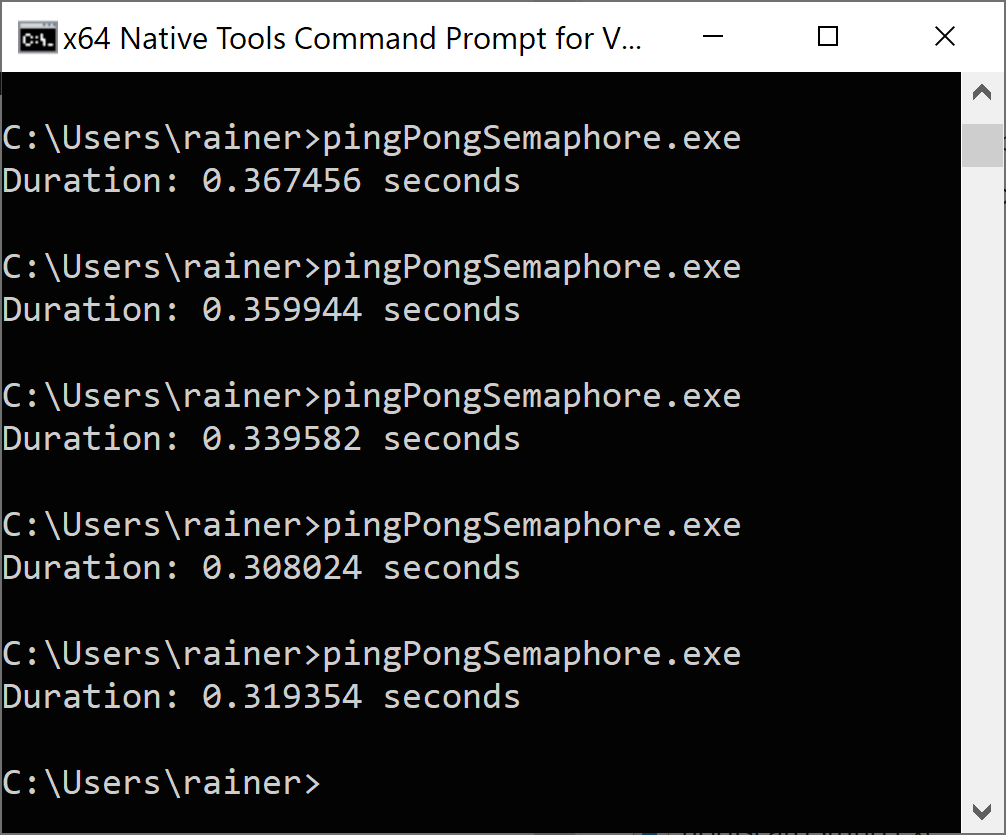
\includegraphics[width=0.8\textwidth]{content/3/chapter7/images/6.png}\\
Multiple time synchronization with semaphores
\end{center}

On average, the execution time is 0.33 seconds.

\subsubsubsection{7.1.5\hspace{0.2cm} All Numbers}

As expected, condition variables are the slowest way, and atomic flag the fastest way to synchronize threads. The performance of a std::atomic<bool> is in between. There is one downside with std::atomic<bool>. std::atomic\_flag is the only atomic data type that is always lock-free. Semaphores impressed me most because they are nearly as fast as atomic flags.

\begin{center}
Execution Time
\end{center}

\begin{table}[H]
\centering
\begin{tabular}{llllll}
&
\textbf{\begin{tabular}[c]{@{}l@{}}Condition\\ Variables\end{tabular}} &
\textbf{\begin{tabular}[c]{@{}l@{}}Two Atomic\\ Flags\end{tabular}} &
\textbf{\begin{tabular}[c]{@{}l@{}}One Atomic\\ Flag\end{tabular}} &
\textbf{\begin{tabular}[c]{@{}l@{}}Atomic\\ Boolean\end{tabular}} &
\textbf{Semaphores} \\ \hline
\textbf{\begin{tabular}[c]{@{}l@{}}Execution \\ Time\end{tabular}} &
0.52 &
0.32 &
0.31 &
0.38 &
0.33
\end{tabular}
\end{table}












